\subsection{Betriebssystemaufteilung}
\begin{frame}{1-Kern-1-System Modell}
	\begin{itemize}
		\item Jeder Kern hat ein Betriebssystem
		\item Flüchtiger Speicher wird partitioniert, jeder Kern bekommt seinen Teil
		\item Restliche Ressourcen geteilt
		\item Problematisch, da Lastausgleich zwischen Kernen unmöglich \(\Rightarrow\) nicht mehr verwendeter Ansatz
	\end{itemize}
\end{frame}

\begin{frame}{Master-Slave Modell}
	\begin{center}
		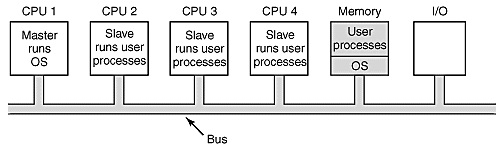
\includegraphics[scale=0.75]{images/assym} \cite{sureshPic}
	\end{center}		
\end{frame}

\begin{frame}{Symmetrisches Modell}
	\begin{center}
		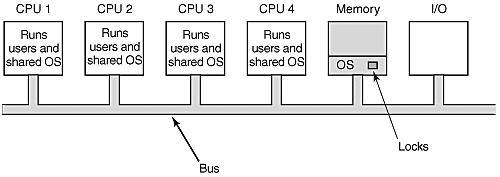
\includegraphics[scale=0.75]{images/symm} \cite{sureshPic}
	\end{center}
\end{frame}

%\subsection{Problem Synchronisation}
%\begin{frame}{}
%\end{frame}

\subsection{MP-Scheduling}
\begin{frame}{Allgemeines}
	\begin{itemize}
		\item Scheduling Strategie bekommt zusätzliche Dimension
		\item Mögliche Aufteilung von Prozessen auf verschiedene Kerne
		\item abhängig von Betriebssystemaufteilung:
		\begin{itemize}
			\item 1-Kern-1-System Modell: Pro Kern ein Scheduler
			\item Master-Slave Model: globaler Scheduler
			\item Symmetrisches Modell: globaler Scheduler
		\end{itemize}
	\end{itemize}
\end{frame}

\begin{frame}{Schedularisierbarkeit}
	\textbf{Optimaler Scheduler:}
	\begin{center}
		\(\sum\limits_{i=1}^{n}\frac{C_i}{P_i} \leq MP\)
	\end{center}
	anstatt:
	\begin{center}
		\(\sum\limits_{i=1}^{n}\frac{C_i}{P_i} \leq 1\)
	\end{center}
	wobei \(MP\) der Anzahl der Prozessoren entspricht
\end{frame}